\section{Unordered Input}
\begin{frame}[c]{Unordered Point Sets}
    \large
    \begin{multicols}{2}
        A set of points $p_i := (x_i, y_i, z_i)$
        $$ \{ p_1, p_2, \ldots, p_n\} $$
        \vspace{1em}
        might be represented by any of its vector permutations $ [ p_{\pi_1}, p_{\pi_2}, \ldots, p_{\pi_n} ] $ for any permutation $\pi$. \\
        \vspace{1em}
        Since point cloud data is \underline{orderless}, it requires
        invariance over input permutations when consumed directly.
        \vspace{2em}
        \begin{figure}
            \centering
            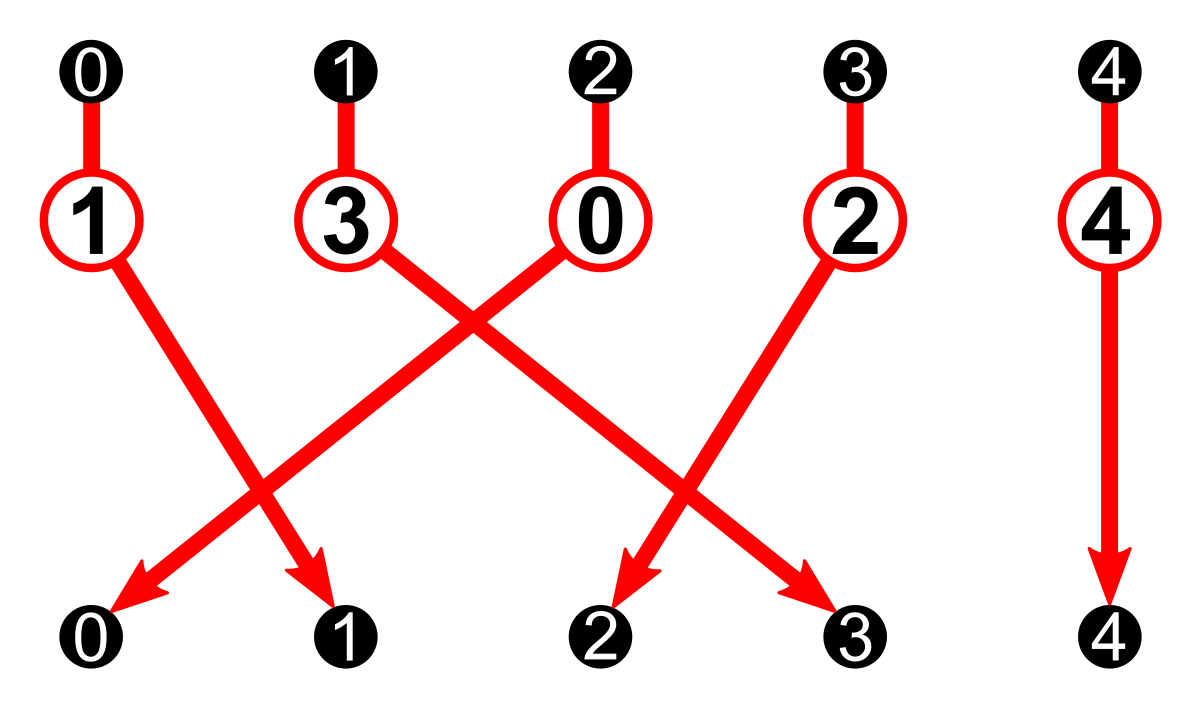
\includegraphics[height=0.4\textheight]{permutation}
            \caption{\textbf{Example Permutation.} \\Figure under CC-BY-SA 4.0 from \cite{BibEntry2022Jun2}}
        \end{figure}
    \end{multicols}
    \pnote{
        Erste Herausforderung: \\
        - umgehen mit beliebigen Eingabe-permutation \\
        - wir verwenden Vektoren um Eingaben darzustellen \\
        - können auch weitere Dimensionen haben \\
        - keine stabile Sortierung der Punkte möglich \\
        - !tricks: neu Messen, anderes Datenset, anderer Sensor \\
        - Mathematisch: tricksen nicht Möglich
    }
\end{frame}


\begin{frame}[c]{Solution: Symmetric Functions}
    \large
    Symmetric functions are invariant over argument permutations $\pi$:
    $$ f(x_1, x_2, \ldots, x_n) \equiv f(x_{\pi_{1}}, x_{\pi_{2}}, \ldots, x_{\pi_{n}}) $$

    \pause

    Examples for symmetric functions:

    \begin{itemize}
        \item $\max$
        \item sum / addition
        \item mean
    \end{itemize}
    \vspace{1em}

    Q: How to integrate a symmetric function into a neural network architecture?
    \pnote{
        Mathematisch: neuronales Netz nur eine Funktion \\
        Funktional betrachtet: Symmetriedarstellung über fkt \\
        \par
        Symmetrisch, wenn Funktionswert bei Argumentenvertausch \\
        gleich bleibt.
        \par
        Es gibt viele Symmetrische Funktionen. Beispiele
        \par
        Frage wird: Wie können eine Symmetrische Funktion in \\
        Architektur von Neuronalem Netz integrieren?
    }
\end{frame}


\begin{frame}[c]{One Symmetric Function is All You Need}
    \large
    A concatenation of functions ($\gamma \circ g(h,..)$) is symmetric if the central function $g$ is symmetric:
    $$ f(x_1, x_2, \ldots, x_n) = \gamma \circ g(h(x_1), \ldots, h(x_n)) $$
    \pause
    \centering
    \begin{figure}
        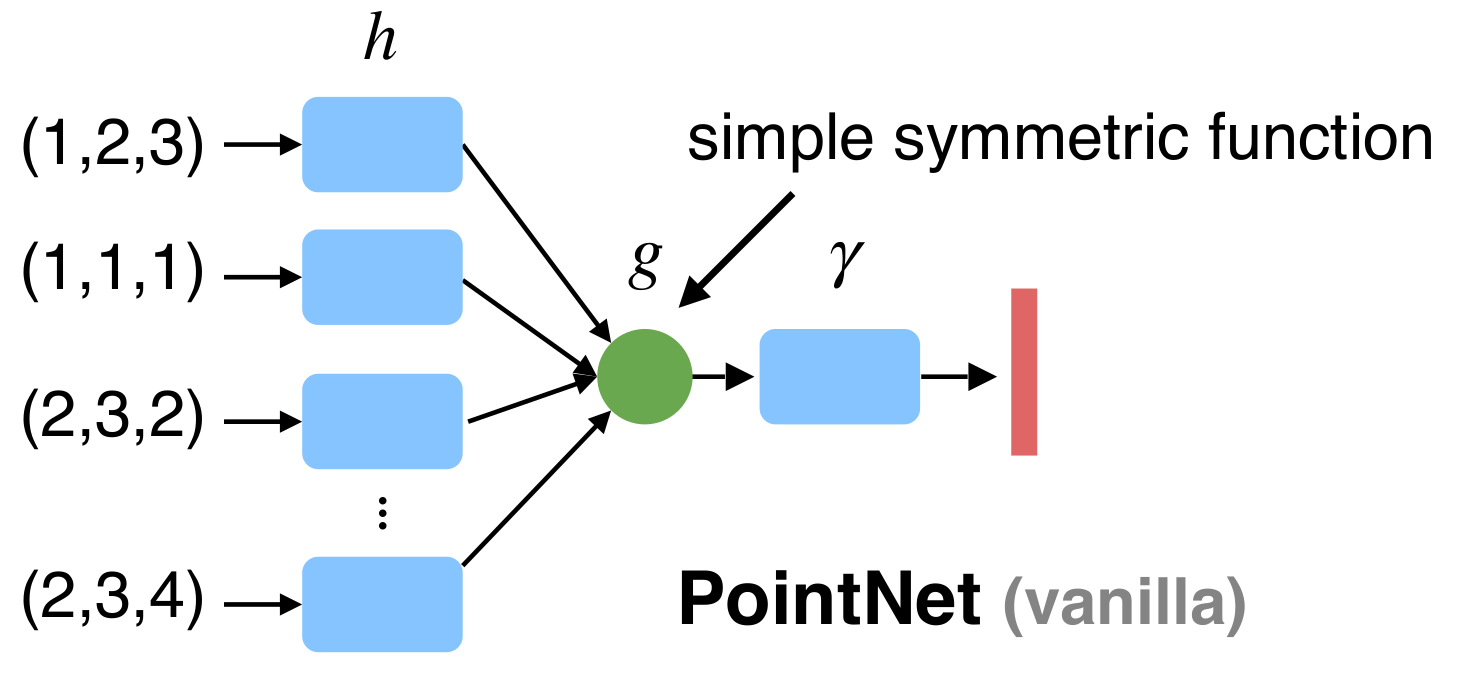
\includegraphics[height=0.45\textheight]{pointnet_vanilla2}
        \caption{Figure from CVPR presentation to \cite{qi2017pointnet}.}
    \end{figure}
    \pnote{
        Erinnerung: Konkatenation von Funktionen kann andere \\
        Funktionen approximieren/darstellen.
        \par
        Konkret können wir mit der konkatenation y o g o h \\
        beliebige symmetrische Funktionen darstellen.
    }
\end{frame}


\begin{frame}[c]{Universal Set Function Approximation}
    \large
    PointNet (vanilla) is a \underline{universal set function approximator}.

    \begin{columns}
        \column{.4\textwidth}
        \begin{greenblock}{Theorem}
            A Hausdorff continuous symmetric function $f: 2^\chi \mapsto \mathbb{R}$ can be arbitrarily approximated by PointNet. \\
        \end{greenblock}
        \column{.4\textwidth}
        \pause
        % $$ \left| f(S) - \underbrace{ \gamma \left( \underset{x_i \in S}{\text{MAX}}\{h(x_i)\} \right)}_{\text{PointNet (vanilla)}} \right| < \varepsilon $$
        $$ \left| f(S) - \underbrace{ \gamma \left( \underset{x_i \in S}{g}\{h(x_i)\} \right)}_{\text{PointNet (vanilla)}} \right| < \varepsilon $$
        with $S \subseteq \mathbb{R}^d$ % and $g :=$ MAX
    \end{columns}
    \vspace{2em}
    For details see \cite{qi2017pointnet} and supplemental material.
    \pnote{
        Bekannt: NN sind allgemeine funktionsapproximatoren \\
        Damit ziemlich trivial: PointNet auch für Permutationen
        \par
        Natürlich braucht eine höhere Genauigkeit mehr Parameter
        \par
        Hausdorff: Topologischer Raum mit disjunkten Nachbarschaften
    }
\end{frame}


\begin{frame}[c]{Basic PointNet Architecture}
    \large
    In practice, both $h$ and $\gamma$ are \textbf{multi-layer perceptrons (MLP)} as generic function approximators.
    Empirically, \textbf{max pooling} provides the best results as symmetric function: \\
    \centering
    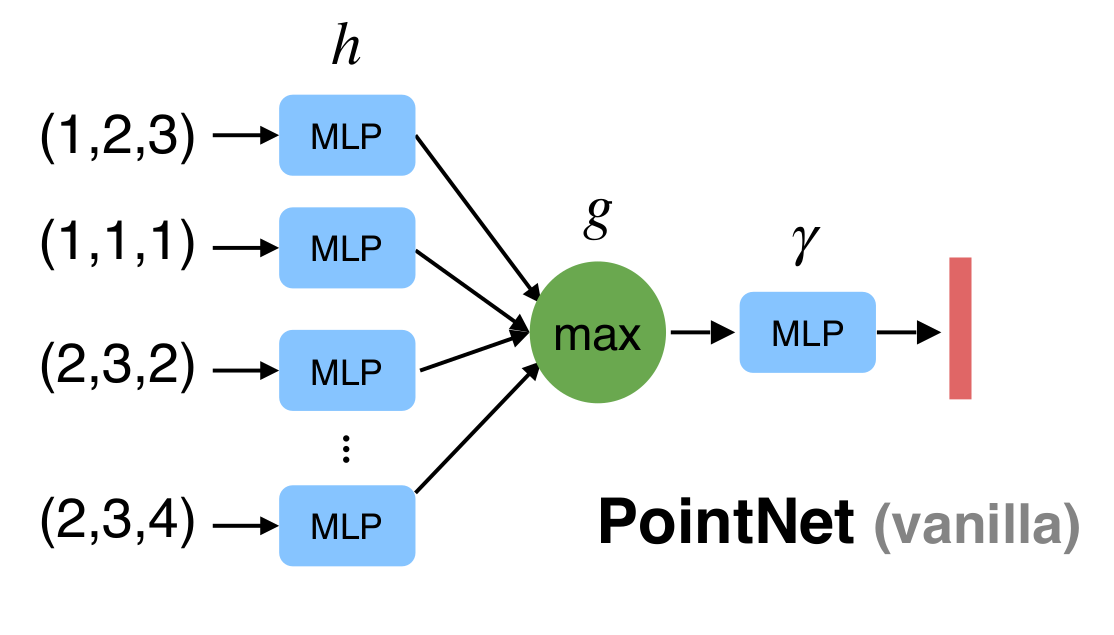
\includegraphics[height=0.6\textheight]{basic_architecture.png}
    \blfootnote{Figure from CVPR presentation to \cite{qi2017pointnet}.}
    \pnote{
        MLP: Dense, Fully-Connected with ReLU \\
        Note that y is shared across all points
        \par
        Andere symmetrische funktionen gehen auch
    }
\end{frame}
